\documentclass{article}


\usepackage{arxiv}

\usepackage[utf8]{inputenc} % allow utf-8 input
\usepackage[T1]{fontenc}    % use 8-bit T1 fonts
\usepackage{hyperref}       % hyperlinks
\usepackage{url}            % simple URL typesetting
\usepackage{booktabs}       % professional-quality tables
\usepackage{amsfonts}       % blackboard math symbols
\usepackage{nicefrac}       % compact symbols for 1/2, etc.
\usepackage{microtype}      % microtypography
\usepackage{lipsum}
\usepackage{amsmath}
\usepackage{graphicx}
\graphicspath{ {./images/} }
\RequirePackage{amsmath,amsthm,amssymb,hyperref} % Math 
\RequirePackage[brazilian]{babel} % Portugûes


\title{Controle e Modelagem de um Motor de Corrente Contínua - Trabalho de Modelagem e Análise de Sistemas Dinâmicos}


\author{
  Docente: Humberto Xavier de Araújo \\
  \And
  Henrique Nunes Poleselo \\
  %% examples of more authors
   \And
 Jesse de O. S. Alves \\
  \And
  Luis Gustavo Christensen
  %% \AND
  %% Coauthor \\
  %% Affiliation \\
  %% Address \\
  %% \texttt{email} \\
  %% \And
  %% Coauthor \\
  %% Affiliation \\
  %% Address \\
  %% \texttt{email} \\
  %% \And
  %% Coauthor \\
  %% Affiliation \\
  %% Address \\
  %% \texttt{email} \\
}
\begin{document}
\maketitle

\section{Introdução}

O ato de medir a velocidade de uma roda, chamado de odometria, é essencial no campo da robótica, principalmente nos dias atuais, onde o poder de processamento tem aumentado, e portanto, possibilitando a fusão de sensores (odometria com visão computacional, por exemplo) para implementação de controladores mais complexos. Dito isso, a aplicação em questão trata da modelagem e controle de velocidade de um motor de corrente contínua que é acoplado a uma roda. Neste relatório serão apresentados alguns métodos utilizados para a obtenção do modelo caixa preta e o processo de elaboração do controlador.
Deste modo, este trabalho está separado em 8 seções onde cada seção está dividida da seguinte forma: na seção 2 serão mencionados os objetivos do projeto, na seção 3 o protótipo é apresentado. Na seção 4 o processo de modelagem é explicitado, na seção 5, o projeto do controlador do sistema. Na seção 6 os resultados obtidos serão apresentados e em seguida após as conclusões do projeto na seção 7. 


\section{Objetivos}
Apesar de utilizar-se os métodos de obtenção de modelo caixa preta, é sabido que ao medir a velocidade angular de um motor de corrente contínua caracteriza um sistema estável. Portanto, o sistema naturalmente chegará ao seu regime permanente. O objetivo da aplicação em questão é fazer com que o motor de corrente contínua atinja esta velocidade angular com um tempo menor utilizando controle PID para reduzir o tempo e o erro.


\section{Descrição do problema}
Para a construção do protótipo utilizou-se apenas um motor de corrente contínua, um Arduino UNO que possui o microcontrolador ATMega328, um sensor (LM393) infravermelho com um fototransistor que gera uma interrupção, um disco de \textit{encoder} e uma ponte H para gerar a corrente necessária para o controle do motor.
A alimentação do motor é dada pela ponte H que recebe um sinal de PWM (\textit{Pulse Width Modulation}) do Arduino e o transmite para o motor com a corrente necessária.
Para obter as curvas da velocidade angular do motor, o disco de \textit{encoder} foi acoplado ao eixo do motor e o sensor infravermelho foi posicionado de modo que este detectasse e gerasse uma interrupção toda vez em que o feixe de onda eletromagnética atravessasse um buraco do disco. Dessa forma, é possível medir a frequência com que o disco gira e utilizando o raio da roda determinar a velocidade angular do mesmo ao longo do tempo. Essas medições realizadas com o sensor foram validadas através de uma marcação na roda e determinação da velocidade linear que posteriormente foi dividida pelo raio da roda, e percebeu-se que o sensor apresenta distorções para rotações altas (próximas a 120 bits de PWM), além de apresentar medições relativamente ruidósas.

Para a leitura da velocidade, fez-se como descrito acima e montado da seguinte forma:
\begin{center}
\centering
  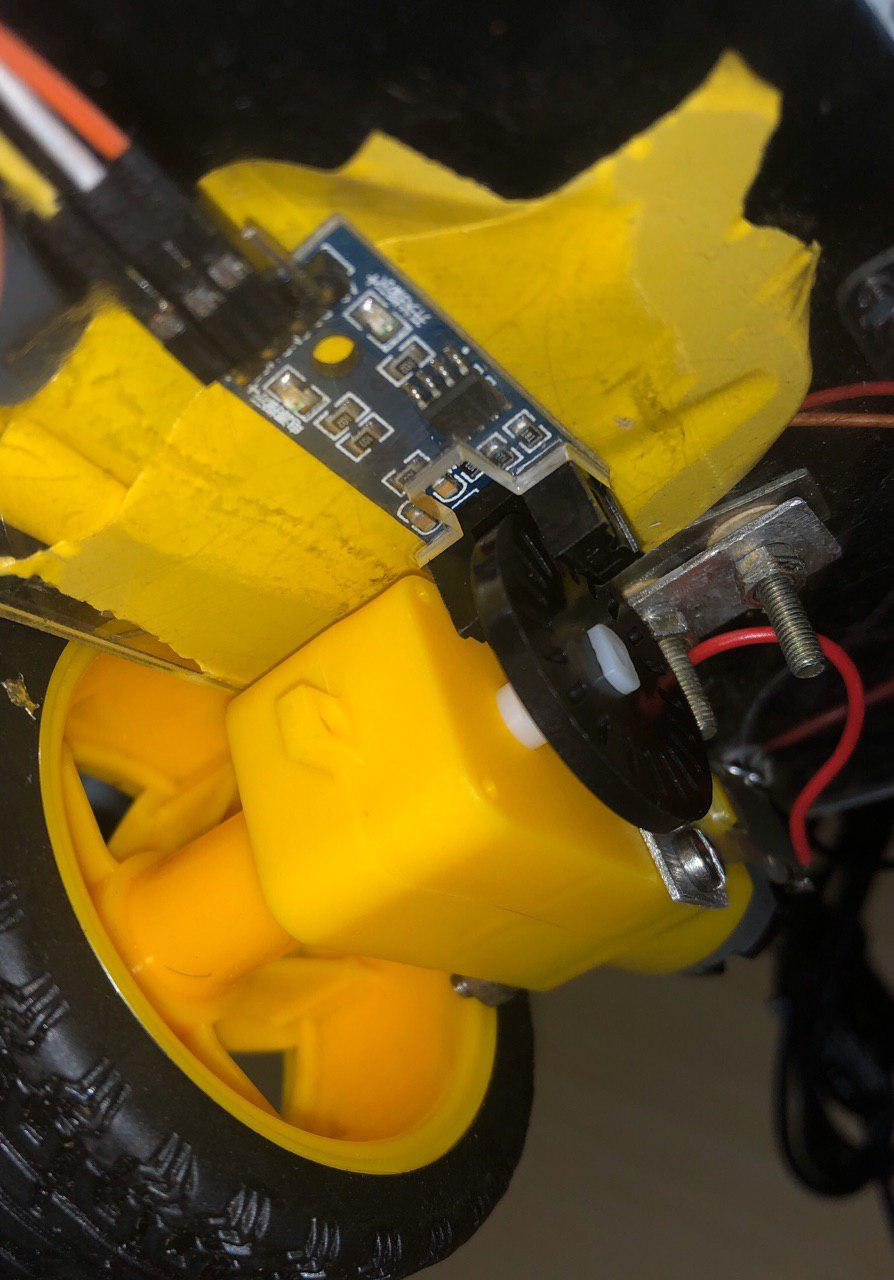
\includegraphics[scale=0.15]{imagens/encoderRoda.jpg}
  
  \caption{Figura 1: Montagem para leitura da velocidade da roda}
\end{center}

Onde as rodas foram acopladas à uma base podendo servir futuramente como um robô. Na seção 4 a modelagem do motor é feita com o robô suspenso, portanto desprezando atrito dinâmico e considerando apenas o atrito estático do próprio motor e da roda. A montagem final pode ser vista na figura

\begin{center}
\centering
  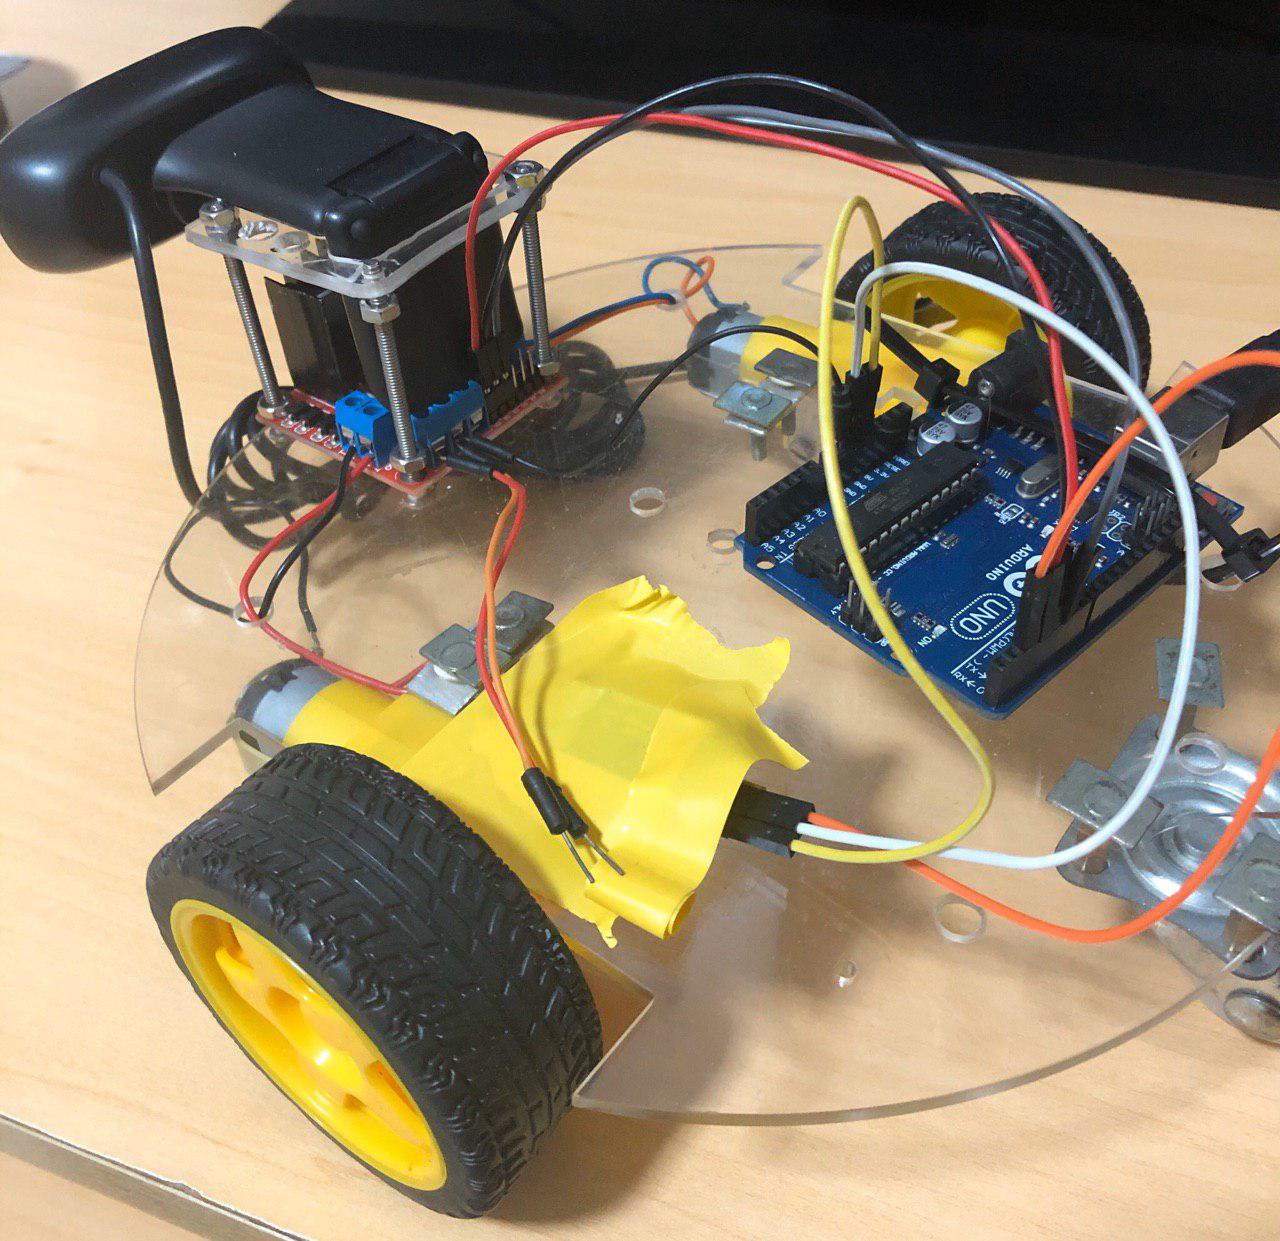
\includegraphics[scale=0.15]{imagens/montagemFinal.jpg}
  
  \caption{Figura 2: Protótipo montado}
\end{center}

\section{Modelagem}


\subsection{Modelo Estático}
Para ter um bom ponto de partida parta a modelagem do sistema, obteve-se a curva do comportamento estático do sistema. Tal curva é importante para determinar a faixa de valores de PWM na qual o sistema responda da forma mais linear, facilitando assim o controle do processo.
Para determinar qual a faixa de operação do PWM, foi aplicado por meio do microcontrolador diferentes valores (de 0 a 255, em bits) e analisou-se que a zona morta do motor se situava na faixa de 0 a 60 bits do PWM, portanto, assumiu-se que a faixa de operação para o controlador seria de no mínimo 6O bits do PWM. O modelo estático foi proposto com a variação do PWM entre 75 e 255 bits pois é a faixa em que o motor opera com segurança.

\begin{center}
\centering
  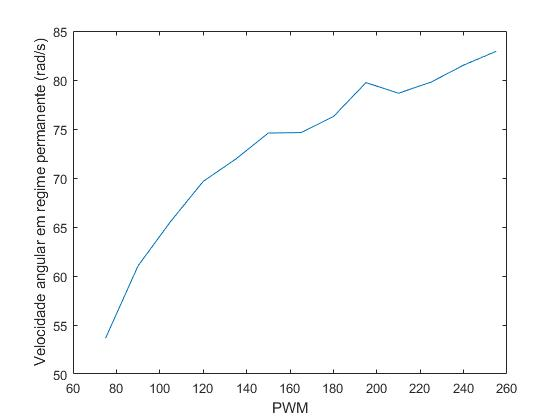
\includegraphics[scale=0.5]{imagens/untitled.jpg}
  
  \caption{Figura 3: Modelo estático do motor de corrente contínua}
\end{center}

A partir da figura 3 é possível notar que na faixa entre 90 e 145 PWM há um comportamento aproximadamente linear, logo é desejável trabalhar com valores contidos nesse intervalo.


\subsection{Modelo Dinâmico}
O modelo dinâmico apresenta a relação entre a entrada e a saída do sistema no regime transitório e permanente. Tal comportamento é obtido a partir de uma entrada degrau, que na aplicação é um "nível DC" do PWM, portanto tensão.
Assim como no modelo estático, a entrada será o valor do PWM e a saída será a velocidade angular da roda. Foi escolhido 120 como valor de PWM já que este se encontra no intervalo em que o sistema mostrou um comportamento linear no modelo estático. Na Figura 4, utilizando a lógica mencionada na seção 3, obteve-se a velocidade angular instantânea da roda com um tempo de amostragem de $50ms$.

\begin{center}
\centering
  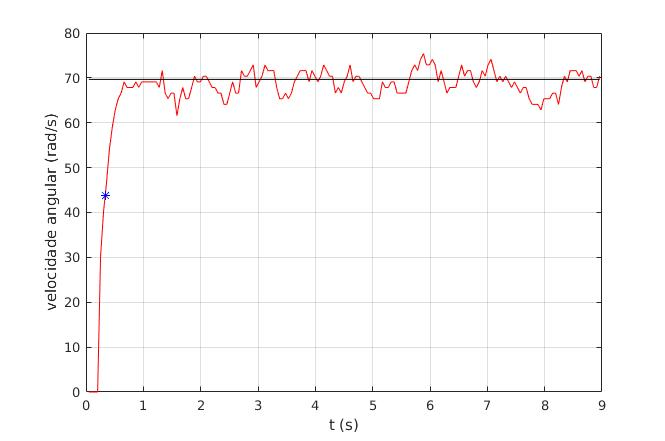
\includegraphics[scale=0.5]{imagens/untitled2.jpg}
  
  \caption{Figura 4: Modelo dinâmico do motor de corrente contínua}
\end{center}

Pela figura 4 é possível ver uma zona morta até o sistema responder, tal fenômeno é devido ao filtro média móvel aplicado posteriormente aos dados da velocidade adquiridos. Viu-se a necessidade de usar filtragem já que o sensor não oferece tanta robustez para altas velocidades. Como no controle optou-se por não usar o filtro média móvel, é possível desprezar a zona morta em questão. No entanto, obteve-se diferentes modelos para efeitos de comparação. A entrada degrau utilizada na figura 4 foi de 120 bits PWM e como é possível inferir pelo gráfico o $y({\infty}) = 69.66 rad/s$  (regime permanente), portanto condizendo com o modelo estático proposto na seção 4.1.

\subsection{Modelo a Dois Parâmetros}
O primeiro modelo proposto foi o de dois parâmetros, o qual utiliza o ganho (K) e a constante de tempo (T) da seguinte forma [1]:

\begin{equation}
    G(s) = \frac{K}{T \cdot s + 1}
\end{equation}

Como sabe-se que $y({\infty}) = 69.66 rad/s$ e a entrada é um PWM de 120 bits, que equivale a $u(t)$ com amplitude de $4.92V$, logo o valor de K é 14.16, que é a divisão entre $y({\infty})$ e a entrada degrau. Para encontrar a constante de tempo, utilizou-se o método da área entre a reta que representa o regime permanente menos a curva de regime transitório [2]. Com o valor da área obtido, o valor de $T$ é encontrado por $T=Ao/k$, onde $Ao$ é a área e $k$ o ganho, portanto $T = 0.2571$. Então:

\begin{equation}
    G(s) = \frac{14.16}{0.2571 \cdot s + 1}
\end{equation}


\subsection{Modelo a Três Parâmetros}
No modelo a três parâmetros, além de utilizar o ganho e a constante de tempo levou-se em conta o atraso $L$ do sistema, de modo a obter o seguinte modelo:

\begin{equation}
    G(s) = \frac{K \cdot e^{-L \cdot s\!}}{T \cdot s + 1}
\end{equation}

O ganho se mantém o mesmo $K = 14.1585$ e o valor do atraso igual ao valor de tempo morto $L = 0.153 s$. Com o valor do atraso e o valor do ganho, obtêm-se a constante de tempo de modo análogo ao obtido com o modelo a dois parâmetros, no entanto considerando o atraso:

\begin{equation}
    T = \frac{Ao}{K} - {L}
\end{equation}

Desse modo, obteve-se $T = 0.1045 s$. Logo o modelo ficou da seguinte forma:

\begin{equation}
    G(s) = \frac{14.1585 \cdot e^{-0.153 \cdot s\!}}{0.1045 \cdot s + 1}
\end{equation}

Utilizando a aproximação linear de Padé(0,1) obteve-se a seguinte função de transferência:

\begin{equation}
    G(s) = \frac{14.1585}{0.0159 \cdot s^{2\!} + 0.2571 \cdot s + 1}
\end{equation}


\subsection{System Identification Toolbox}
Além dos modelos obtidos acima, utilizou-se a \textit{toolbox} do MATLAB \textit{System Identification}, na qual utiliza os dados de saída e entrada para a obtenção do modelo.

Com 2 pólos e zeros infinitos:
\begin{equation}
    G(s) = \frac{1186}{s^{2\!} + 16.49 \cdot s + 84.71}
\end{equation}

Com 1 pólo e zeros infinitos:
\begin{equation}
    G(s) = \frac{65.36}{s + 4.656}
\end{equation}

Utilizando a função \textit{step} às funções de transferência (2), (6), (7) e (8) foi obtida a resposta ao degrau de $4.92V$:

\begin{center}
\centering
  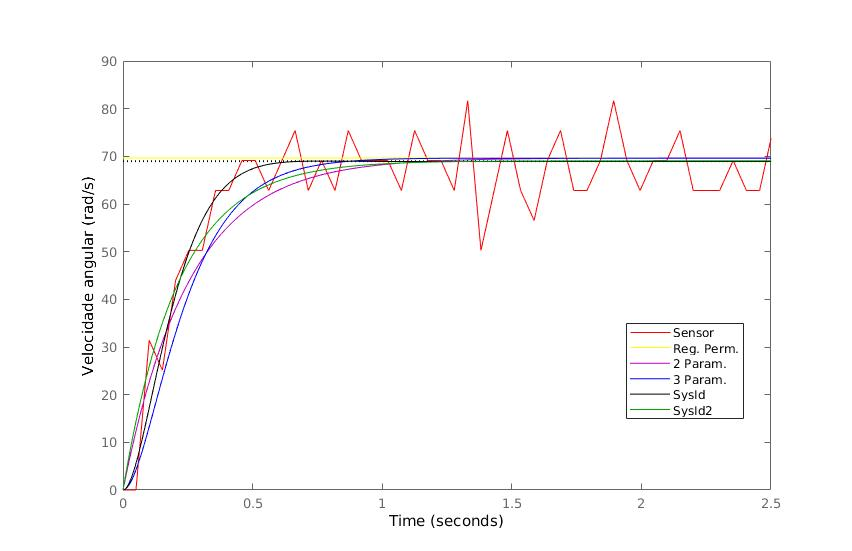
\includegraphics[scale=0.5]{imagens/respaoDegrauLinda2Rel.jpg}
  
  \caption{Figura 5: Gráfico para diferentes aproximações da função de transferência do motor}
\end{center}

Vale notar que o filtro média móvel foi retirado de forma a tirar o atraso e poder comparar as curvas de forma mais fidedigna. Uma boa métrica para escolher as melhores funções de transferência seria calculando o erro entre a curva experimental (vermelha) e as respectivas funções aproximadas e ver qual possuí o menor erro. Infelizmente não houve tempo durante o experimento realizado para tal, portanto foi utilizada a métrica de quais curvas parecem mais se aproximar da vermelha, que são as curvas rosa e azul, respectivamente as aproximações (2) e (3).
Para validar as escolhas feitas foi simulado na ferramenta \textit{Simulink} todas as funções aproximadas e com o critério de Routh para estabilidade testou-se os ganhos $Kp$, $Ki$ e $Kd$ para ver como os sistemas se comportavam em malha fechada. No final das contas, o próprio $Simulink$ conta com um atalho para à ferramenta \textit{PID Tuner}, que busca ganhos que provém robustez ao sistema (rejeição de ruído e seguimento de referência), portanto utilizando a ferramenta viu-se que os modelos escolhidos conseguiam prover uma boa resposta, como será visto mais a frente.

\section{Projeto do Controlador}
Como foram escolhida duas aproximações para o sistema, propõe-se dois controladores. Portanto, foi calculada a função de transferência em malha fechada da aproximação (2):

\begin{equation}
    \frac{Y(s)}{R(s)} = \frac{s^{2\!} \cdot {14.1585 \cdot Kd} + s \cdot {14.1585 \cdot Kp} + {14.1585 \cdot Ki}}{s^{2\!} \cdot {(0.2517+14.1585 \cdot Kd)} + s \cdot {(14.1585 \cdot Kp + 1)} + {14.1585 \cdot Ki}}
    \end{equation}
    
    Aplicando o critério de Routh para obter o intervalo em que os ganhos do controlador geram um sistema estável, foi obtido $Kd > -0.0178$, $Kp > -0.0706$ e $Ki > 0$. Sabendo o intervalo de valores em que os ganhos devem estar contidos. Como mencionado anteriormente, foi simulado \textit{PID Tuner} juntamente com o \textit{Simulink} para obter os ganhos com certa robustez para o controlador, sendo tais ganhos: $Kp = 0.094472$, $Ki = 0.734462$ e $Kd = -0.000882$ onde todos os ganhos obedecem às condições impostas pelo critério de Routh, portanto estes foram utilizados no projeto do PID. Portanto, a função de transferência ficou da seguinte forma:
    
    \begin{equation}
    \frac{Y(s)}{R(s)} = \frac{s^{2\!} \cdot {-0.0125} + s \cdot {1.3376} + {10.3989}}{s^{2\!} \cdot {0.2392} + s \cdot {2.3376} + {10.3989}}
    \end{equation}
    
    A função de transferêcia obtida gerou a seguinte curva:
    
    \begin{center}
    \centering
        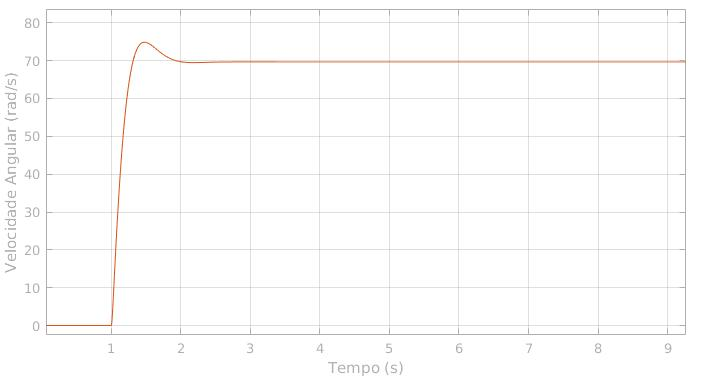
\includegraphics[scale=0.5]{imagens/PID2Param.jpg}
        
        \caption{Figura 6: Resposta do sistema (2) em malha fechada com controlador PID no Simulink}
    \end{center}
    
    Ao fazer o procedimento análogo ao último porém com o modelo a três parâmetros, foi observado que o \textit{PID Tuner} do MATLAB retornou valores dos ganhos no PID que resultaram num sinal de controle inviável fisicamente (saturação), ao remover o ganho derivativo foi observado que o sinal de controle se tornou viável de ser gerado, portanto foi decidido utilizar um controlador PI nesse caso. Ao fechar a malha do controlador PI com o modelo a três parâmetros (6), foi obtido a seguinte função de transferência:
    
    \begin{equation}
    \frac{Y(s)}{R(s)} = \frac{s \cdot {14.1585 \cdot Kp} +  {14.1585 \cdot Ki}}{s^{3\!} \cdot {0.016} s^{2\!} \cdot {0.26} + s \cdot {(14.1585 \cdot Kp + 1)} + {14.1585 \cdot Ki}}
    \end{equation}
    
    Realizando novamente o critério de Routh, obteve-se os seguintes intervalos dos ganhos $Kp > -0.07$ e $0 < Ki < Kp + 17.26$. Como os ganhos que a ferramenta \textit{PID Tuner} retornou estão contidos nesse intervalo, os mesmos foram utilizados sendo $Kp = 0.1341$ e $Ki = 0.7349$. Desta forma obteve-se a seguinte função de transferência em malha fechada:
    
     \begin{equation}
    \frac{Y(s)}{R(s)} = \frac{s \cdot {1.8987} +  {10.4051}}{s^{3\!} \cdot {0.016} + s^{2\!} \cdot {0.26} + s \cdot {2.8987} + {10.4051}}
    \end{equation}
    
    A função de transferência obtida gerou a seguinte curva:
    
    \begin{center}
    \centering
        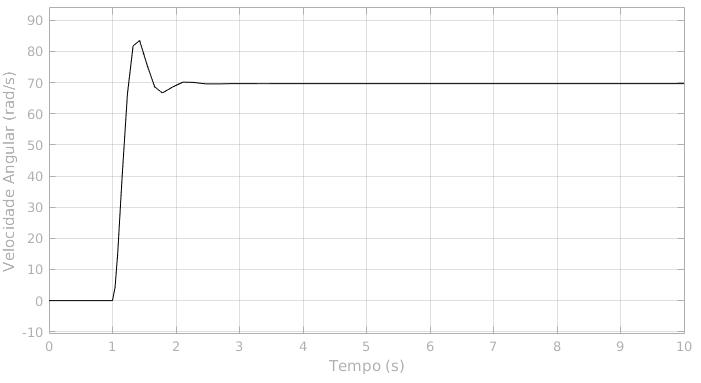
\includegraphics[scale=0.5]{imagens/PID3Param.jpg}
        
        \caption{Figura 7: Resposta do sistema (6) em malha fechada com controlador PI no Simulink }
    \end{center}
    
    Os ganhos "ótimos" retornados pelo \textit{PID Tuner} foram: (consequentemente os usados nos experimentos)
    \begin{center}
    \begin{tabular}{|c|c|c|c|c|}
            \hline
            Modelo & $Kp$ & $Ki$ & $Kd$ & Controlador \\
            \hline
            (2) & 0.094471 &  0.73446 & -0.000882 & 1 \\
            \hline
            (6) & 0.134078, & 0.73489 & 0 & 2 \\
            \hline
    \end{tabular}
    
  \caption{Quadro 1}
\end{center}
    

    
\section{Resultados experimentais}

Para melhor avaliar os controladores propostos é interessante avaliar qual controlador provê o menor erro, portanto uma boa métrica para se utilizar é o \textit{Integral of the Square of the Error} ou ISE, é basicamente elevar cada elemento do vetor erro ao quadrado depois soma-los [3].

\begin{center}
    \begin{tabular}{|c|c|c|c|}
            \hline
            PWM (bits) & $ISE$ (rad^2/s^2) & Controlador & Modelo \\
            \hline
            120 & $9.3345*10^4$ & Não & X \\
            \hline
            75 & $8.7627*10^4$ & Não & X \\
            \hline
            120 & $8.8662*10^4$ & 1 & (2) \\
            \hline
            75 & $1.0561*10^4$ & 1 & (2)\\
            \hline
            120 & $1.0534*10^5$ & 2 & (6) \\
            \hline
            75 & $9.9548*10^3$ & 2 & (6)\\
            \hline
    \end{tabular}
    
  \caption{Quadro 2}
\end{center}

Pelo Quadro 1 infere-se que o melhor controlador foi o PID com o modelo (6), pois apresentou o menor erro. É interessante notar que para alta velocidade (alto PWM) as medidas começam a ter muita inconsistência e portanto mesmo com o controlador o erro não diminui, isso deve-se principalmente ao sensor.

Para tentar melhor avaliar o controlador adicionou-se um distúrbio ao sistema de forma a tirar o mesmo de sua referência, novamente usou-se como métrica o $ISE$:

\begin{center}
    \begin{tabular}{|c|c|c|}
            \hline
            PWM (bits) & ISE (rad^2/s^2) & Controlador \\
            \hline
            120 & $1.2112*10^5$ & 1 \\
            \hline
            75 & $2.6285*10^4$ & 1\\
            \hline
            120 & $1.3101*10^5$ & 2\\
            \hline
            75 & $2.4900*10^4$ & 2\\
            \hline
    \end{tabular}
    
  \caption{Quadro 3}
\end{center}

Outra métrica para analisar se a presença do controlador nesse sistema é desenhar os gráficos da velocidade do motor com a roda quando: não há controlador, com o controlador, com o controlador com distúrbio externo, assim fez-se para o PWM de 120 bits, i.e referência de $59.66rad/s$:

\begin{center}
    \centering
        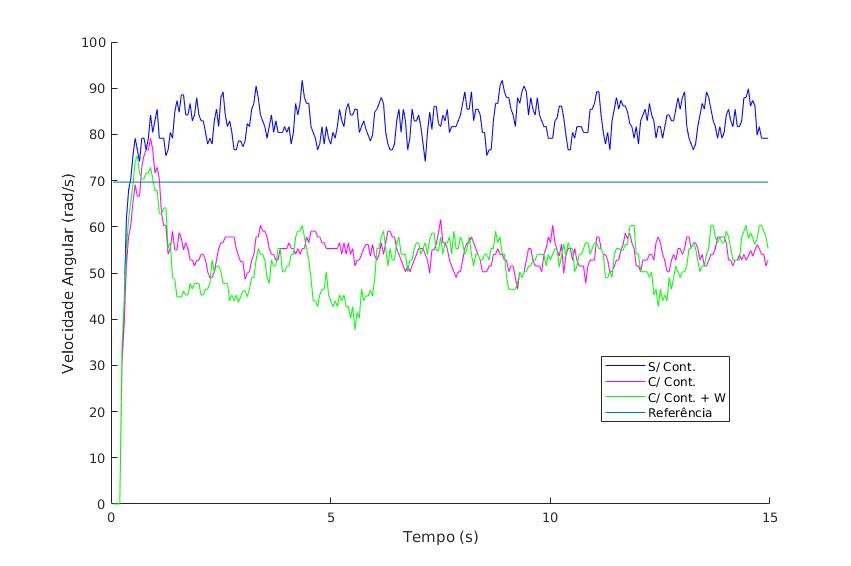
\includegraphics[scale=0.5]{imagens/pwm120.jpg}
        
        \caption{Figura 8: Resposta do sistema sem controlador, com controlador e com controlador + distúrbio }
\end{center}

\begin{center}
    \centering
        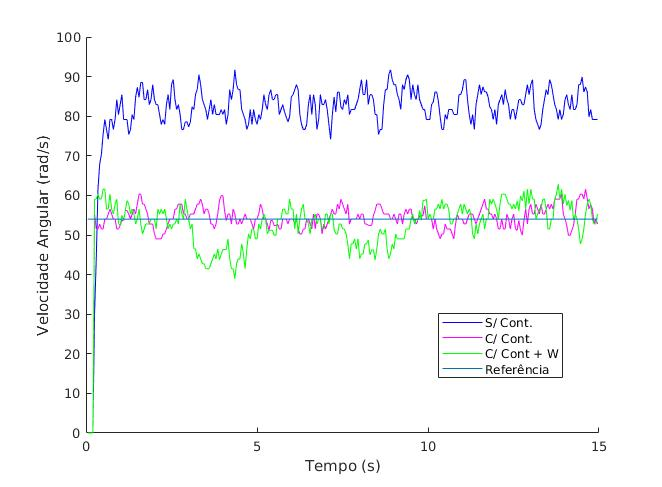
\includegraphics[scale=0.5]{imagens/pwm75.jpg}
        
        \caption{Figura 9: Resposta do sistema sem controlador, com controlador e com controlador + distúrbio }
\end{center}

Quando a velocidade da roda é menor (54 rad/s) faz com que o sensor consiga trabalhar em uma faixa melhor, portanto é infere-se da figura 9 que a curva rosa de fato fica em torno da referência (reta azul), e mesmo com distúrbios ao sistema (curva em verde) o mesmo fica em torno da referência. Percebe-se que a falta do controlador de fato faz diferença, já que a curva em azul está totalmente fora da referência.

Já com a velocidade maior (com 69.66 rad/s) ou 120 bits de PWM percebe-se que há muitos erros associados às medidas, resultando na velocidade de referência estar completamente distoante da velocidade real, seja com o o controlador ou sem.


\section{Conclusão}
Após as leituras dos dados experimentais e obtenção de dois modelos, juntamente com a variação do PWM entre os valores de 120 e 75 bits, percebe-se que quanto maior o sinal de PWM maior são os erros,i.e , em altas velocidades ocorrem problemas de precisão na leitura dos sensores. Além de que o modelo a dois parâmetros com um PWM de 75 bits fornece o menor erro quadrátio e isso se deu pelo fato de estar em rotações mais baixas e do ganho $Kd$ ser diferente de zero (somente no modelo a dois parâmetros), fazendo-o responder mais rapidamente.

Os códigos tanto para os cálculos analíticos quanto o da implementação da lógica do controlador no Arduino podem ser encontrados no seguinte link: \url{https://github.com/hpoleselo/ssfr}


\bibliographystyle{unsrt}  
%\bibliography{references}  %%% Remove comment to use the external .bib file (using bibtex).
%%% and comment out the ``thebibliography'' section.


%%% Comment out this section when you \bibliography{references} is enabled.
\begin{thebibliography}{1}
\bibitem{hadash2018estimate}
Control System Design by Karl Johan Aestroem

\bibitem{kour2014real}
Código Fonte MATLAB, Autoria Própria.
\newblock https://github.com/hpoleselo/SSFR/tree/master/PlantModel/WheelModel.

\bibitem{kour2014fast}
\newblock Dorf, R. C.; Bishop, R. h. Sistemas de Controle Moderno. 5a edição



\end{thebibliography}


\end{document}
